\documentclass[11pt]{article}
\usepackage[margin=.75in]{geometry}
\usepackage[all]{xy}

\usepackage{amsmath,amsthm,amssymb,color,latexsym}
\usepackage{mathtools}
\usepackage{geometry}
\usepackage{booktabs}
\geometry{letterpaper}    
\usepackage{graphicx}
\usepackage{tabto}
\usepackage{setspace}
\usepackage[dvipsnames]{xcolor}

\usepackage[noframe]{showframe}
\usepackage{framed}

\renewenvironment{shaded}{%
  \def\FrameCommand{\fboxsep=\FrameSep \colorbox{shadecolor}}%
  \MakeFramed{\advance\hsize-\width \FrameRestore\FrameRestore}}%
 {\endMakeFramed}
\definecolor{shadecolor}{gray}{0.90}

\newtheorem{problem}{Problem}

\newenvironment{solution}[1][\it{Solution:}]{\textbf{#1 } }

\onehalfspacing

\begin{document}
\begin{titlepage}
   \begin{center}
       \vspace*{9cm}

       \textbf{CS 332 Fall 2025}

       \vspace{0.5cm}
        Project \#1
        \vfill

       \textbf{Koshi Harashima, Ben Cole}\\
       Due Date: 10/8, 2025
            
   \end{center}
\end{titlepage}

\pagebreak

%%%%%%%%%%%%%%%%%%%%%%%%%%%%%%%%%%%%%%%%%%%%%%%%%%%%%%%%%%%
%%%%%%%%%%%%%%%%%%%%%%%% Problems %%%%%%%%%%%%%%%%%%%%%%%%%
%%%%%%%%%%%%%%%%%%%%%%%%%%%%%%%%%%%%%%%%%%%%%%%%%%%%%%%%%%%

%--------------------------------------------------------
\begin{problem}
\end{problem}

\begin{shaded}
\subsection*{Method}
For each value $v\!\in\!\{10,\dots,100\}$ and bid $b$, the winning probability is
\[
P_{\text{win}}(b)=P(\text{opp}<b)+\tfrac12P(\text{opp}=b),
\qquad
EU_{\text{exact}}(v,b)=(v-b)P_{\text{win}}(b).
\]
In the exact calculation, the opponent bid distribution is the empirical class distribution:
a value is chosen uniformly from $\{10,\dots,100\}$ and a random classmate’s bid for that value is drawn; ties are broken uniformly at random.
The Monte Carlo (MC) estimate samples 20,000 such random opponent bids and averages realized utilities.
The optimal bid $b^*(v)$ maximizes $(v-b)P_{\text{win}}(b)$.

\subsection*{Results}
Regret is defined as the difference between the optimal expected utility and your own expected utility at each value.

\vspace{1em}
\textbf{Ben's case}
\begin{center}
\small
\begin{tabular}{@{}rrrrrrrr@{}}
\toprule
value & my bid & win prob & EU exact & EU MC & opt bid & opt EU & regret \\
\midrule
 10 &   9 & 0.091 & 0.091 & 0.088 &  5 & 0.334 & 0.243 \\
 20 &  15 & 0.216 & 1.080 & 1.075 & 11 & 1.740 & 0.660 \\
 30 &  20 & 0.291 & 2.909 & 2.865 & 11 & 3.694 & 0.785 \\
 40 &  25 & 0.375 & 5.625 & 5.569 & 21 & 6.529 & 0.904 \\
 50 &  30 & 0.455 & 9.091 & 9.089 & 21 & 9.984 & 0.893 \\
 60 &  30 & 0.455 &13.636 &13.633 & 31 &14.713 & 1.076 \\
 70 &  35 & 0.532 &18.614 &18.648 & 31 &19.804 & 1.190 \\
 80 &  40 & 0.607 &24.273 &24.406 & 41 &25.462 & 1.189 \\
 90 &  45 & 0.677 &30.477 &30.651 & 41 &32.007 & 1.530 \\
100 &  50 & 0.745 &37.273 &37.403 & 51 &38.675 & 1.403 \\
\bottomrule
\end{tabular}
\end{center}
Average regret (opt EU - my EU): \textbf{0.98}.

\newpage

\vspace{1em}
\textbf{Koshi's case}
\begin{center}
\begin{tabular}{@{}rrrrrrrr@{}}
\toprule
value & my bid & win prob & EU exact & EU MC & opt bid & opt EU & regret \\
\midrule
 10 &   9 & 0.091 & 0.091 & 0.088 &  5 & 0.334 & 0.243 \\
 20 &  19 & 0.252 & 0.252 & 0.250 & 11 & 1.740 & 1.487 \\
 30 &  29 & 0.418 & 0.418 & 0.417 & 11 & 3.694 & 3.276 \\
 40 &  39 & 0.577 & 0.577 & 0.580 & 21 & 6.529 & 5.952 \\
 50 &  49 & 0.716 & 0.716 & 0.718 & 21 & 9.984 & 9.268 \\
 60 &  59 & 0.805 & 0.805 & 0.806 & 31 &14.713 &13.908 \\
 70 &  69 & 0.855 & 0.855 & 0.856 & 31 &19.804 &18.949 \\
 80 &  79 & 0.905 & 0.905 & 0.904 & 41 &25.462 &24.557 \\
 90 &  89 & 0.950 & 0.950 & 0.951 & 41 &32.007 &31.057 \\
100 &  99 & 0.991 & 0.991 & 0.991 & 51 &38.675 &37.685 \\
\bottomrule
\end{tabular}
\end{center}
Average regret (opt EU - my EU): \textbf{14.63}.


\subsection*{Takeaways}
\begin{itemize}
\item Exact and Monte Carlo expected utilities closely align, confirming simulation accuracy.  
\item Optimal bids shade below value and rise smoothly with $v$, matching first-price auction theory.  
\item Ben’s bids were close to optimal (avg regret was about 1 util); Koshi’s near-truthful bids overpaid and reduced utility.
\item A good strategy is to choose, for each value $v$, the $b$ that maximizes $(v-b)\Pr[\text{opp}<b]$ using the empirical opponent distribution.  
\end{itemize}
\end{shaded}
\pagebreak


%-------------------------------------------
\begin{problem}
\end{problem}

\begin{shaded}
\subsection*{Method}
\begin{itemize}
  \item \textbf{(1) Data-driven bid:} From \texttt{bid\_data.csv}, estimate the win CDF $F_v(b)=\Pr(B_{\text{opp}}\le b\mid v)$ and choose $\hat b^*(v)=\arg\max_{0\le b\le v}(v-b)\,\hat F_v(b)$.
  \item \textbf{(2) Bid in Theory:} Two-bidder first-price: assume opponent bids linearly $b_{\text{opp}}=\alpha X$ and choose $b$ to maximize $U(b\mid v)=(v-b)\Pr(\text{win at }b)$
\end{itemize}

\pagebreak

\subsection*{Result}


\begin{itemize}
  \item \textbf{(1) Data-driven bid:} More samples $\Rightarrow$ more accurate $\hat F_v$ and higher expected profit than with few samples.
  \item \textbf{(2) Bid in Theory:} The optimal bid is $v/2$, consistent with the optima recovered from the sample.
\end{itemize}

\subsection*{Takeaways}
\begin{itemize}
  \item \textbf{More simulation means more accurate results.} (With many runs, simulated profit matches the exact calculation.)
  \item \textbf{Bid below your value; about half is a good rule of thumb.} (With two similar bidders, the math says bid $\approx v/2$.)
\end{itemize}
\end{shaded}


% Figures
\centering
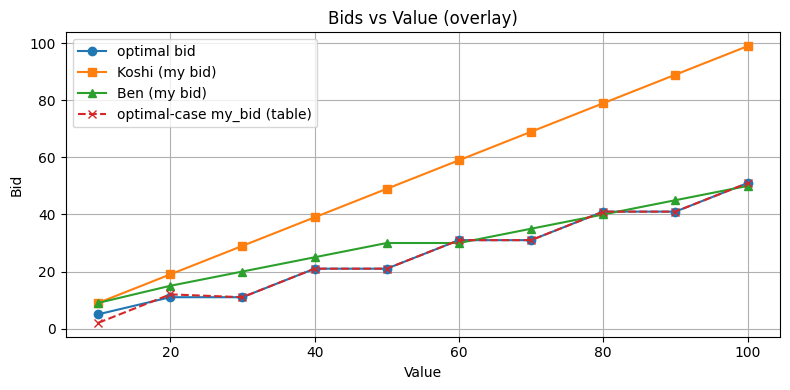
\includegraphics[width=1\linewidth]{332Project1/figures/bid.png}
\vspace{0.4em}
{\footnotesize (a) Bid vs.\ value}

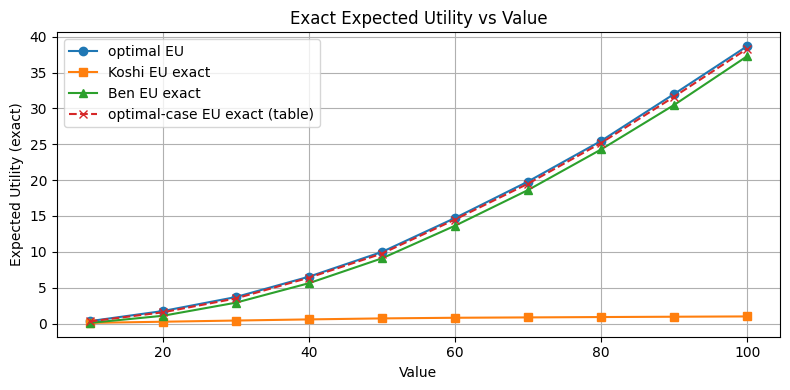
\includegraphics[width=1\linewidth]{332Project1/figures/utility.png}
\vspace{0.4em}
{\footnotesize (b) Expected utility vs.\ value}

\end{document}